\xchapter{Avaliação da disponibilidade dos softwares científicos de análise estática}
{Este capítulo apresenta a avaliação e caracterização dos softwares científicos
de análise estática de código fonte quanto à sua disponibilidade ou
sustentabilidade técnica, ou seja, a capacidade de perdurar, de continuar
disponível no futuro.}
\label{caracterizacao-ferramentas}

% Introduction
% Background
% Experimental Setup (hipoteses / design)
% Results (data analysis)
% Discussion
% Threats to validity
% Conclusions

Muitos estudos em engenharia de software sofrem de dificuldades de repetição
\cite{Tang2016}, uma prática importante para aumentar a validade científica dos
estudos e seus resultados. {\it Repetição} é a atividade de refazer exatamente
o que outra pessoa fez usando os artefatos originais, a disponibilidade de
código fonte é o requisito mínimo para possibilitar tal prática.

Avaliar e caracterizar a disponibilidade dos {\it softwares cientificos}
publicados em conferências de engenharia de software, com especial atenção à
disponibilidade do seu código fonte, é útil para evidenciar o quão possível é
repetir tais estudos e assim aumentar a validade em seus resultados.

Sabe-se que artigos que citam o desenvolvimento de scripts ou protótipos
apresentam chance próximo a nulo de ter estes artefatos disponíveis
publicamente e terem seu código fonte acessível. A replicabilidade tende a cair
com a idade do paper, uma das razões é que as páginas web onde os softwares e
possivelmente dados são publicados tem uma grande chance de se tornarem
indisponíveis ao passar do tempo \cite{robles2010replicating}.

O recente Dagstuhl Manifesto \cite{allen2017engineering} indica como futura
direção de pesquisa quantificar a disponibilidade de softwares científicos, e
sugere a seguinte questão de pesquisa: Na literatura científica publicada, como
as taxas de softwares disponíveis, executáveis, e escondidos ({\it hidden
software}) mudam ao longo do tempo?

Alinhado à esta sugestão de investigação, o atual trabalho define como objetivo
geral avaliar a disponibilidade dos softwares científicos publicados em
conferências de engenharia de software e assim evidenciar o quanto tais estudos
sofrem com dificuldades de repetição.

Esta avaliação e caracterização será focada em publicações da área de análise
estática de código fonte visto que seria inviável no escopo deste trabalho
englobar todas as áreas de pesquisa da engenharia de software.

A área de análise estática de código fonte possui carência de estudos avaliando
suas ferramentas, desta forma conseguiremos contribuir com esta área ao mesmo
tempo que exploramos o quanto os pesquisadores publicando softwares nesta área
publicam e disponibilizam seus softwares contribuindo para a divulgação dos
resultados e proporcionam repetição dos seus estudos.

\section{Planejamento do estudo}

\subsection{Questões de pesquisa}

Neste estudo temos as seguintes questões de pesquisa, adaptados para o contexto
de análise estática de código fonte, a partir das sugestões de investigação
apresentadas no Dagstuhl Manifesto \cite{allen2017engineering}:

\newcommand{\QuestaoUm}{Os softwares que nós usamos e produzimos no contexto
acadêmico de análise estática de código fonte é sustentável?}

\newcommand{\QuestaoDois}{Na literatura científica publicada, como as taxas de
softwares disponíveis, do domínio de aplicação de análise estática, mudam ao
longo do tempo?}

\newcommand{\QuestaoTres}{Podemos adaptar de forma incremental o softwares
científicos de análise estática para aproveitar oportunidades emergentes, sem
perda de reprodutibilidade e sem custos proibitivos?}

\begin{description}
  \item [Q1:] \QuestaoUm
  \item [Q2:] \QuestaoDois
  \item [Q3:] \QuestaoTres
\end{description}

\subsection{Seleção de softwares científicos}

Selecionamos softwares via {\it revisão estruturada}, um processo disciplinado
para busca e seleção de softwares de um domínio específico publicados em
artigos acadêmicos a partir de critérios bem definidos, de forma que seja
possível a reprodução do estudo por parte de pesquisadores interessados.

A revisão estruturada difere da revisão e do mapeamento sistemático
\cite{Kitchenham2007} por ser um processo mais simples e menos rígido, onde o
resultado final é um conjunto de softwares, enquanto no mapeamento ou na
revisão sistemática há um esforço em caracterizar os artigos analisados o mesmo
não ocorre na revisão estruturada, onde o esforço está em caracterizar os
softwares científicos.

A revisão estruturada é organizada em três atividades de (1) busca de artigos
(definição das fontes, obtenção dos artigos nas fontes), (2) filtro (definição
de critérios de busca, definição de script de busca) e (3) seleção de artigos
com publicação de softwares. Estas atividades estão representadas na Figura
\ref{figura-revisao-estruturada}.

\begin{figure}[h]
  \center
  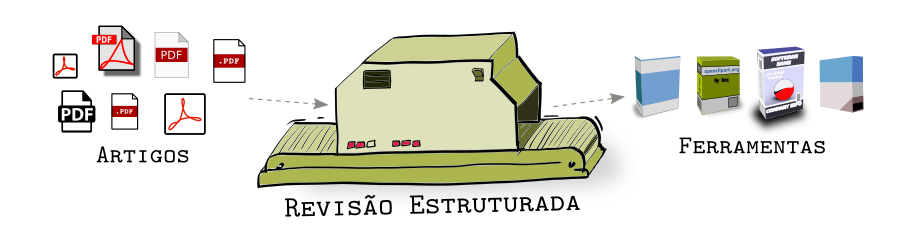
\includegraphics[scale=0.21]{imagens/revisao-estruturada.png}
  \caption{Atividades da revisão estruturada}
  \label{figura-revisao-estruturada}
\end{figure}

O resultado final da revisão estrutuda é um conjunto de softwares científicos e
informações sobre em qual artigo foi publicado, qual conferência e ano o artigo
foi publicado e em quais fontes o software pode ser obtido, geralmente páginas
web, repositórios de código fonte ou outros endereços na internet. Cada
atividade da revisão estruturada é detalhada à seguir:

\begin{description}

  \item[(1) Busca]
    A primeira atividade da revisão estruturada define as fontes de entrada,
    estas fontes são conferências que abordam o tema de interesse do estudo, e
    que apresentam um grande potencial de encontrar softwares do domínio de
    aplicação desejado, neste estudo o interesse está em softwares de análise
    estática de código fonte, portanto as conferências selecionadas serão
    aquelas com potencial de se encontrar softwares deste domínio de aplicação.
    Esta primeira atividade deve incluir o maior número possível de ediçoes de
    cada conferência, para cada edição é copiado localmente todos os artigos em
    formato PDF para filtro na atividade 2.

  \item[(2) Filtro]
    A segunda atividade da revisão estruturada realizada em cima de todo o
    conjunto de artigos selecionados na etapa anterior é um filtro automático
    que busca em todo o conteúdo dos artigos os termos de interesse, estes
    termos devem ser pensados em relaçao ao domínio de aplicação desejado,
    devem ser abrangentes a fim de evitar falsos negativos, ou seja, evitar que
    o filtro deixe de fora artigos que publiquem software de análise estática,
    mesmo que isto gere alguns falsos positivos, a atividade seguinte irá
    identificar os falsos negativos deixando-os fora do resultado final da
    revisão. Os seguintes termos serão utilizados neste filtro:

    \begin{verbatim}
      "tool" OU "framework"; E
      "download" OU "available"; E
      "http" OU "ftp"; E
      "static analysis" OU "parser".
    \end{verbatim}

    Esses termos devem encontrar artigos com publicação de softwares
    científicos do domínio de análise estática de código fonte com
    disponibilidade para {\it download}, seja binário ou código fonte, será
    aplicado automaticamente com auxílio de um script desenvolvido durante este
    trabalho de pesquisa, detalhes deste script, outros artefatos produzidos durante esta
    pesquisa, e onde obtê-los pode ser encontrado no Apêndice \ref{reproducibilidade-do-estudo}.

  \item[(3) Seleção]
    A terceira e última atividade da revisão estruturada identifica se cada
    artigo resulta, de fato, em publicação de software científico do domínio de
    aplicação desejado. Esta seleção é feita a partir de uma leitura
    superficial do artigo em busca de indícios de que o artigo publica de fato
    algum software.

    Para cada artigo é lido, título, introdução, resultados
    e conclusões com o objetivo de identificar se o artigo publica software
    científico e indica onde obter uma cópia do software. Quando esta leitura inicial
    não é suficiente para identificar se há publicação de software, outras seções são
    lidas, alguns artigos descrevem a implementação do software em seções específicas,
    outros indicam detalhes do software ao longo de todo o texto, é comum o uso
    de notas de rodapé para indicar onde o software está disponível. Softwares científicos
    que sejam mais abrangentes do que apenas análise estática de código fonte
    mas que contenham esta função em seu conjunto também são selecionados.

\end{description}

Ao final das 3 atividades da revisão estruturada é gerado como saída um
conjunto de softwares científicos de análise estática de código fonte, para
cada software teremos o nome, descrição e em qual artigo o software foi
publicado, além da informação sobre a fonte para obtenção do software.

\subsection{Quantificação da disponibilidade dos softwares científicos}

Os softwares científicos selecionados na revisão estruturada foram avaliados em
relação à sua disponibilidade, apenas os softwares com indicação de fonte para
obtenção foram incluídos aqui, dois aspectos foram analisados.

O primeiro relacionado à como o artigo disponibiliza o software científico
avalia se de fato o software está disponível, ou seja, se a fonte informada
para obtenção está funcional e acessível publicamente, será caracterizado entre
uma das seguintes opções:

\begin{itemize}
  \item Fonte para obtenção do software indisponível:\\
    {\it O artigo indica fonte mas encontra-se inacessível, fora do ar ou com erros}
  \item Software disponivel, binários ou código fonte\\
    {\it A fonte indicada está disponível e acessível publicamente}
\end{itemize}

A fonte indicada será acessada a fim de identificar se está funcional e se é
possível obter uma cópia do software. Este é um requisito fundamental para
conseguir responder à questão de pesquisa {\bf Q1:} \QuestaoUm

%Mesmo que o autor tenha disponibilizado fontes para obtenção dos artefatos produzidos,
%o fato de não informarem a fonte inviabiliza, ou ao menos dificulta, bastante
%pesquisadores interessados em repetir ou reproduzir os resultados de tais estudos.

Esta questão diz respeito à sustentabilidade técnica, a capacidade de perdurar
e continuar disponível no futuro. O segundo aspecto diz respeito à como o
software está disponível, é um nível de detalhe sobre o primeiro aspecto, os
softwares caracterizados como disponíveis no primeiro aspecto serão detalhados
aqui, informando de que forma estão disponíveis, se código fonte, ou apenas
binários.

\begin{itemize}
  \item Código fonte disponível
  \item Apenas binários disponível
\end{itemize}

%Esse segundo aspecto toma como base o trabalho de \citeonline{Novak2010} em que
%propõe uma taxonomia e um conjunto de dimensões para caracterização de
%ferramentas de análise estática, uma das dimensões para caracterização
%é esta relacionado à como o software é disponibilizado.

Lembrando que apenas os softwares caracterizados no primeiro aspecto como
{\it``software disponivel, binários ou código fonte''} serão detalhados aqui.
Os softwares caracterizados como {\it ``código fonte disponível''} incluirão
qualquer softwares mesmo sem licença definida, não estamos avaliando neste
momento se o software é livre ou aberto segundo as definições de software {\it
livre} e {\it open} da Free Software
Foundation\footnote{\url{https://www.gnu.org/philosophy/free-sw.html}} e Open
Source Initiative\footnote{\url{https://opensource.org/osd}}, respectivamente,
o acesso ao código fonte é a característica de interesse neste estudo, com ele
é possível estudar o conhecimento empregado nos softwares, bem como repetir o
estudo original utilizando ou executando tal código quando necessário.

A fonte para coleta dessas informações serão os artigos relacionados aos
softwares, código fonte, documentos e site do projeto, quando disponíveis.

\section{Resultados}

Na revisão estruturada selecionamos a conferência SCAM - {\it
Source Code Analysis and Manipulation Working
Conference}\footnote{\url{http://www.ieee-scam.org}} e a conferência ASE - {\it
Automated Software Engineering}\footnote{\url{http://ase-conferences.org}},
ambas conferências com largo histórico de publicação sobre análise de
programas e apresentam um alto potencial de encontrar softwares do domínio de
análise estática de código fonte.

A primeira atividade da revisão estruturada -- (1) Busca -- passa por
todas as ediçoes das duas conferências até o ano de 2015, ou seja, explora o
histórico de 24 anos de publicação. Todas as trilhas de ambas as conferências
foram incluídas, encontramos nesta atividade 1873 artigos no total, 1527 artigos
do ASE e 346 artigos do SCAM, com uma média geral de 75 artigos publicados por ano. A
Figura \ref{artigos-por-ano} apresenta a distribuição por edição de cada
evento.

\begin{figure}[h]
  \center
  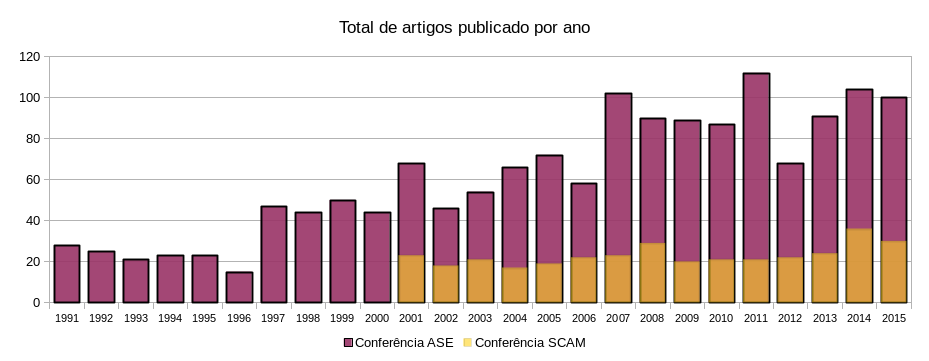
\includegraphics[scale=0.65]{imagens/artigos-por-ano.png}
  \caption{Gráfico em barras com o total de artigos publicado por ano}
  \label{artigos-por-ano}
\end{figure}

Entre os anos de 1991 e 1996 a conferencia ASE chamava-se KBSE - {\it
Knowledge-Based Software Engineering Conference} e só a partir de 1997 passou a
chamar-se ASE - {\it Automated Software Conference}. A edição com o maior
número de publicações foi 2011 com 112 artigos publicados, seguido de 2014 com
104, e 2007 com 102, a edição com o menor número foi 1996 com apenas 15 artigos
publicados.

A conferência SCAM teve sua primeira edição apenas em 2001, 10 anos após a
primeira edição do ASE, e possui uma média de 23 artigos publicados por edição.
Se compararmos os mesmos períodos de ambas as conferências, 2001 à 2015,
percebemos que a conferência ASE publica quase 4 vezes mais do que a
conferência SCAM. Neste período a conferência ASE teve uma média de 80 artigos
publicados por ano, se for levado em conta todas as edições, apenas da
conferência ASE, a média cai para 61 artigos por ano.

A segunda atividade da revisão estruturada -- (2) Filtro -- reduziu em 77\%
o número total de artigos de forma automática a partir da string de busca, resultando em 441 artigos
para serem analisados na próxima etapa da revisão estruturada.  Durante a execução desta
atividade foi necessário analisar dois artigos manualmente, {\it Adaptable
concern-based framework specialization in UML} e {\it Property-oriented test
generation from UML Statecharts}. O conteúdo destes dois artigos não é possível
de ser analisados pelo script de filtro uma vez que é formado por imagens
digitalizadas, ambos artigos publicados no ASE edição 2004. Nenhum dos dois
artigos continham os termos pesquisados e ficaram fora do conjunto selecionado
nesta atividade.

A terceira e última atividade da revisão estruturada -- (3) Seleção --
realizada em cima dos 441 artigos selecionou 107 artigos com publicação de
software científico do domínio de aplicação de análise estática, alguns destes
artigos fazem referência à um mesmo software, é o caso do {\it BEST: A symbolic
testing tool for predicting multi-threaded program failures} e do {\it Scalable
and precise symbolic analysis for atomicity violations}, ambos publicados no
ASE 2011 fazem referência ao software BEST. Situação similar ocorreu com o {\it Augmenting
Counterexample-Guided Abstraction Refinement with Proof Templates} e o {\it
PtYasm: Software Model Checking with Proof Templates} publicados no ASE 2008,
fazem referência ao software PtYasm. Por conta disso, entre os 107 artigos, temos
105 softwares distintos, uma lista com todos os softwares e uma breve descrição
de cada um é apresentado no Apêndice \ref{resumo-softwares},
detalhes sobre o número de artigos e softwares encontrados em cada conferência
pode ser consultados nos Apêndices \ref{artigos-do-scam} e \ref{artigos-do-ase} 

Ainda durante esta atividade da revisão cada um dos 107 artigos foram
analisados em busca de informações sobre onde encontrar o software indicado,
esta análise resultou em 60 softwares com indicação de fonte para obtenção do
software, todos os artigos indicam endereço de página web para download do
software. A Figura \ref{softwares-disponivel-por-ano} apresenta estes 60
softwares distribuídos ao longo dos anos num gráfico em linha.

\begin{figure}[h]
  \center
  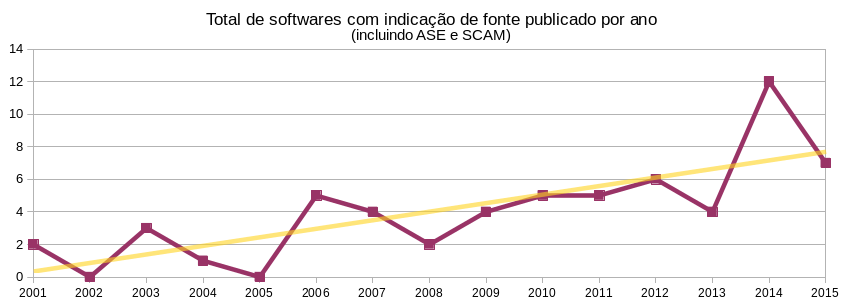
\includegraphics[scale=0.65]{imagens/softwares-por-ano.png}
  \caption{Gráfico em linha com o número de softwares por ano selecionados na revisão estruturada}
  \label{softwares-por-ano}
\end{figure}

Apesar da busca na atividade -- (2) Filtro -- utilizar termos com o objetivo de
encontrar apenas softwares disponíveis com informação de onde encontrar o
software, ainda assim, encontramos 45 artigos com publicação de software sem
indicação de fonte para obtenção.

Entre os 1873 artigos, encontramos 107 artigos referenciando 105 softwares de
análise estática, apenas 60 destes indicam fonte onde o software pode ser
encontrado, apenas 37 estão disponíveis, os 23 restantes indicam fonte não mais
acessíveis, endereço não encontrado, indisponível, ou com informações não
relacionadas ao software. O Apêndice \ref{resumo-softwares-disponiveis} traz
uma tabela com os nomes e endereços web onde os softwares estão disponíveis.

Esta informação nos permite responder a questão de pesquisa {\bf Q1:}
\QuestaoUm

Levando em conta a sustentabilidade técnica podemos responder que 61\% dos
softwares produzidos no domínio de aplicação de análise estática são
sustentáveis, ou seja, continuam disponíveis ao longo do tempo. Lembrando que
não está sendo considerado aqui pesquisas que publicam software sem menção à
fonte onde pode ser encontrado, a revisão estruturada teve como foco encontrar
artigos com publicação softwares com indicação de fonte, ou seja, aqueles
artigos que publicam software mas que não indicam fonte não está sendo
considerado aqui, vimos que na revisão estruturada, mesmo não sendo o objetivo
encontramos 45 artigos sem informação de fonte, isto faria esta taxa cair para
apenas 35\%, uma revisão estruturada mais abrangente com objetivo de encontrar
todo e qualquer software, independente de indicar fonte ou não, com certeza
faria esta taxa cair abaixo dos 35\%.

\citeonline{robles2010replicating} afirma que existe uma tendência das páginas
web onde os softwares estão disponíveis tem uma grande chance de se tornarem
indisponíveis ao passar do tempo, podemos investigar esta tendência 
avaliando os 60 softwares com fonte indicada no artigo,
identificar se confirmamos neste contexto se com a idade do paper
as páginas web onde os softwares são publicados tem uma grande chance de se
tornarem indisponíveis ao passar do tempo.

\begin{figure}[h]
  \center
  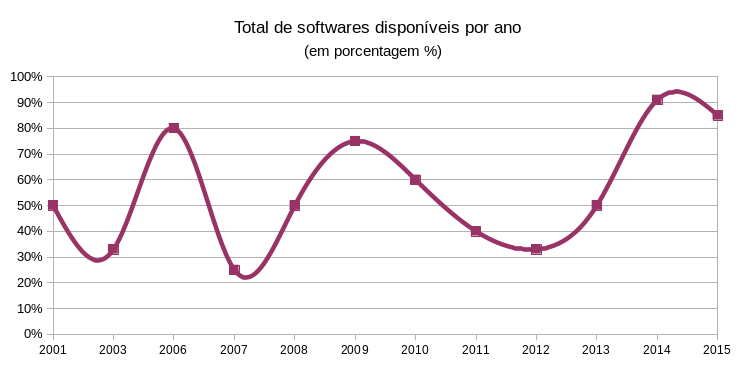
\includegraphics[scale=0.65]{imagens/softwares-disponivel-por-ano.png}
  \caption{Gráfico em linha com o total de softwares disponíveis por ano}
  \label{softwares-disponivel-por-ano}
\end{figure}

A Figura \ref{softwares-disponivel-por-ano} apresenta em cada ano quantos
porcentos do total de softwares publicados com indicação de fonte estão ainda continuam
disponíveis hoje, ou seja, quantos qual é a taxa de softwares que continuam
disponíveis hoje dentro do conjunto de softwares publicados em cada ano com
informação sobre fonte para download.  Os anos de 2002, 2004, 2005, e
anteriores a 2001 não possuem softwares publicados com fonte indicada no artigo
ainda disponível, portanto não constam no gráfico suas informações.

Ao analisar a figura percebemos que há um leve crescimento na disponibilidade
dos softwares nos anos mais recentes, com isso podemos responder à nossa
questão de pesquisa {\bf Q2:} \QuestaoDois

Existe uma leve tendência da fontes informadas, páginas web, se tornarem
indisponível ao longo do tempo, é possível notar que em 2006 80\% de todos os
softwares de análise estática publicados estão ainda disponíveis, este número
cresce em 2014 chegando a 90\%, e cai no ano seguinte para 85\%, apesar de não
estar sempre crescente, e de termos uma amostra pequena, apenas 60 softwares,
este leve indício confirma a afirmação de \citeonline{robles2010replicating}.

Esses 37 softwares com fonte disponível foram avaliados em relação ao segundo
aspecto em respeito à de que forma estão disponíveis, os artigos informam onde
obter tais softwares, os softwares estão realmente disponíveis, as fontes
indicadas foram acessadas e na presente data deste trabalho estão funcionando e
acessíveis, mas queremos saber em qual formato estes softwares estão
disponíveis?

\begin{itemize}
  \item Código fonte disponível
  \item Apenas binários disponível
\end{itemize}

Entre estes apenas 3 não possuem código fonte disponível, 34 estão com o código
fonte disponível publicamente, dentre elas 13 não informam licença alguma
apensar de ter o código fonte disponível, 21 informam licenças de FOSS ({\it
free and open source software}):
8 usam GNU General Public License;
2 usam Apache License;
4 usam BSD License;
3 usam Eclipse Public License;
2 usam University of Illinois/NCSA Open Source License;
1 usa licença {\it FrontEndART Software Ltd}; e
1 usa licença {\it SAnToS Laboratory Open Academic License}.

Com essas informações podemos responder à terceira e última questão de
pesquisa desse estudo {\bf Q3:} \QuestaoTres

Entre os 37 softwares disponíveis 21 podem ser modificados para se adaptar às
necessidades emergentes sem necessidades de solicitação prévia de autorização
aos autores originais devido ao uso de licenças livres. Os 13 softwares
restantes com código fonte disponível mas sem licença expressa podem
eventualmente serem modificados mas a falta de uma licença impõe à necessidade
de solicitar permissão aos autores originais.

35\% dos softwares disponíveis podem ser adaptados de forma incremental para
aproveitar oportunidades emergentes, 21\% podem mediante prévia autorização do
autor original serem modificados, e apenas 5\% não oferecem essa possibilidade
por não disponibilizarem o código fonte publicamente.

\section{Ameaças à validade}

Estamos considerando que o código fonte é necessário para repetir um dado
estudo mas pode ser que em alguns casos o estudo possa ser repetido mesmo sem a
disponibilidade do mesmo, isto poderia ser resolvido realizando a repetição
de cada estudo na prática e a partir daí identificar se o código fonte dos
softwares desenvolvidos são requeridos.

A escolha de um domínio de aplicação específico para seleção dos softwares
pode ser um fator de influencia nos resultados obtidos, sendo possível que
o número de artigos com publicação de softwares com código fonte disponível
encontrado não reflita nos outros domínios, os problemas diagnosticados
neste domínio pode não ser verdade em outros domínios, sendo necessário
realizar o mesmo estudo em outros domínios.

A leitura dos artigos na revisão estruturada para identificar se publicam
softwares de análise estática de código fonte, se disponibilizam fonte para
obtenção de tais softwares, e se os softwares são mesmo do domínio de aplicação
de análise estática de código fonte podem ter maior validade se feitos em
par e revisados por outros pesquisadores, neste estudo tudo foi feito pelo
autor deste estudo e não houve revisão por pesquisadores independentes.

\section{Conclusões}

Dos 346 artigos do SCAM e 1533 artigos do ASE analisados na revisão estruturada
apenas 44\% (155 artigos) e 18\% (281 artigos) continham os termos pesquisados
no filtro automático da segunda atividade da revisão, respectivamente.

Deste total apenas 11\% (41 artigos) e 4\% (62 artigos) foram selecionados na
terceira e última atividade da revisão contendo publicação de ferramenta de
análise estática.

Resultando em 103 artigos com publicação de {\it software científico} de
análise estática de código fonte, apenas 35 possuem fonte para obtenção do
software, sendo 32 de código aberto, ou seja, com disponibilidade de
código fonte, e 3 grátis, apenas binários disponível. Ou seja, apenas 31\% dos
artigos com publicação de software disponibilizam o código fonte das mesmas.
Isto significa que 69\% dos artigos com publicação de software de análise
estática de código fonte são potencialmente impossíveis de serem repetidos, já
que os artefatos originais são necessários para tal atividade e o artigo não
disponibiliza o código fonte dos mesmos.

% o artigo com resumo do RESER 2011 diz \cite{knutson2010report}:
% 4) Re-
% search tools are either not available or not usable, so precise
% replication is impractical [1, 2, 8, 18, 19].

Muitos outros aspectos podem ser levados em consideração quando se está
avaliando a capacidade de repetir ou replicar um estudo, aqui avaliamos apenas
a disponibilidade de código fonte dos softwares científicos, mas inúmeros detalhes
pormenores são necessários, tais como: indicar qual versão do software foi
utilizado no estudo, 

No entando, consideramos que nem todos os scripts e código fonte pode
valer o custo de dua publicação, sabe-se que umas das barreiras para publicação
de muitos destes artefatos são as dificldades em tal atividade,
e as objeções a tal prática de ter RR reques um esforço adicional \cite{madeyski2017would},
em muitos
estudos o simples fato de não possuir código disponível pode não levar
a problemas para alcançar a meta final que é aumento da validade do estudo,


Todas as atividades e artefatos produzidos neste estudo estão documentados em
repositório público no
Github\footnote{\url{http://github.com/joenio/dissertacao-ufba-2016}}, o
Apêndice \ref{apendice-revisao-estruturada} traz mais informações.

%, uma lista completa e
%o endereço de cada edição onde os artigos foram obtidos está documentado no
%Apêndice \ref{edicoes-conferencias}

% IDEIA!
% levantar ano de publicação do artigo para cada software e
% calcular por quanto tempo cada software está disponível,
% com isso verificar se há um padrão, ou seja, se publicações
% mais antigas possuem softwares não-disponíveis, obsoletos,
% etc...
